\section{Results}
\label{sec:results}

\subsection{The benchmark requires memory (RQ1)}
\label{sec:res_bench}
Episodes last 300 to 1000 control steps with 2--5 picks (Table~\ref{tab:dataset}), while a pick, from contact to detachment, occupies only about a dozen frames. A leaf-hidden fruit is invisible in a median 78\% of the frames in which it still hangs on the tree, two-thirds of the hidden fruits are ripe, and in FruitCount the basket is never in the front view. Neither task can be solved from the current frame: the policy must remember where hidden ripe fruits are and how many fruits it has picked.

\subsection{Picking events from the tool-to-fruit distance (RQ2, RQ3)}
\label{sec:res_events}
\label{sec:res_robust}
\emph{Detection is exact over a physically determined plateau.} Events detected from the ground-truth distance have precision, recall and F1 of exactly 1.000 for every radius between 1 and 4~cm, on the training set (where $r$ was selected) and the validation set, with the correct pick count in every validation episode (Fig.~\ref{fig:events}a; all radii in Supplementary Table~S2). At 0.5~cm the gripper does not always come that close (recall 0.628); beyond half the inter-fruit spacing, approaches to neighbouring fruits merge into spurious events (count exact 0.49 at 10~cm). The contact keyframe precedes detachment by a median of 4 frames and the release keyframe coincides with it. On the 200 perturbed DART-H demonstrations, precision is 0.998, recall 1.000 and the count is exact in 99\% of episodes.

\emph{Robustness yields an accuracy specification for perception.} Table~\ref{tab:robust} and Fig.~\ref{fig:events}b--d report detection on corrupted validation distances (5 seeds per level): white Gaussian noise, correlated Ornstein--Uhlenbeck noise, independent and contiguous dropouts (runs averaging 10 frames) and a constant bias. Independent dropouts are nearly harmless (F1 1.000 with 30\% of frames missing, since unknown frames inherit the last state), and a bias of $-1$ to $+2$~cm, as from a miscalibrated depth camera, leaves the count exact. White noise is the main threat: at 1~cm the plain detector's F1 falls to 0.846 and the count is exact in only 37\% of episodes, because the distance chatters around the threshold. Both filters remove this (F1 0.999, count exact 99\%); hysteresis does so without delay, keeping 0.995 of the K4 keyframes against 0.980 for the median filter, and is more robust to correlated noise (F1 0.953 versus 0.941 at 2~cm), so it is the default deployment detector. Long contiguous dropouts covering a whole approach remain the weak case (F1 0.894--0.913). With hysteresis, distance errors of up to 1.5~cm white noise (F1 0.987) or 2~cm correlated noise (F1 0.953) keep the event F1 above 0.95: this is the accuracy specification for any perception module that feeds \pekm.

\begin{table}[t]
\centering
\caption{Robustness of event detection and K4 memory to perturbations of the validation distance signal (5 seeds per level). Each cell: plain / median5 / hysteresis. Keyframe recall: fraction of clean-signal keyframes found within $\pm3$ frames in the perturbed memory.}
\label{tab:robust}
\footnotesize
\begin{adjustbox}{max width=\textwidth}\begin{tabular}{llccc}
\toprule
Perturbation & Level & Event F1 & Count exact & Keyframe recall (K4)\\
\midrule
None & -- & 1.000 / 1.000 / 1.000 & 1.00 / 1.00 / 1.00 & 1.000 / 1.000 / 1.000\\
White noise & 0.5 cm & 0.971 / 1.000 / 1.000 & 0.86 / 1.00 / 1.00 & 0.985 / 0.989 / 0.997\\
White noise & 1 cm & 0.846 / 0.999 / 0.999 & 0.37 / 0.99 / 0.99 & 0.932 / 0.980 / 0.995\\
White noise & 2 cm & 0.635 / 0.969 / 0.947 & 0.03 / 0.85 / 0.78 & 0.846 / 0.966 / 0.958\\
Correlated (OU) & 2 cm & 0.887 / 0.941 / 0.953 & 0.58 / 0.74 / 0.79 & 0.918 / 0.926 / 0.931\\
Independent dropout & 30\% & 1.000 / 1.000 / 0.998 & 1.00 / 1.00 / 0.99 & 0.998 / 0.999 / 0.996\\
Independent dropout & 50\% & 0.996 / 0.996 / 0.988 & 0.98 / 0.98 / 0.94 & 0.982 / 0.987 / 0.973\\
Contiguous dropout & 30\% & 0.913 / 0.913 / 0.894 & 0.62 / 0.62 / 0.55 & 0.882 / 0.901 / 0.867\\
Bias & $-1$ cm & 1.000 / 1.000 / 1.000 & 1.00 / 1.00 / 1.00 & 0.998 / 0.999 / 0.999\\
Bias & $+2$ cm & 1.000 / 1.000 / 1.000 & 1.00 / 1.00 / 1.00 & 1.000 / 1.000 / 1.000\\
\bottomrule
\end{tabular}\end{adjustbox}
\end{table}

\begin{figure}[t]
\centering
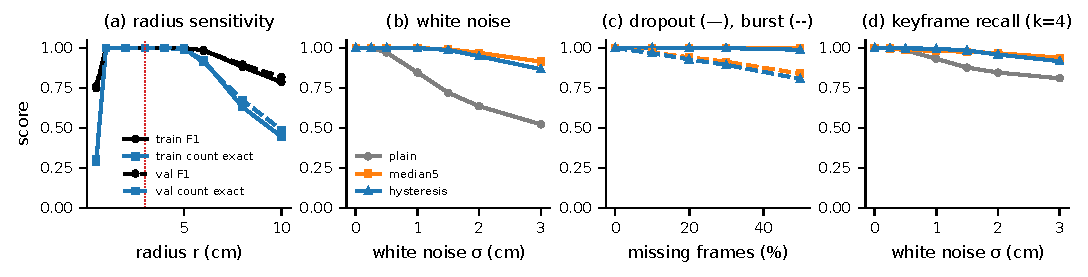
\includegraphics[width=\linewidth]{fig6_event_detection}
\caption{Event detection. (a) F1 and count exact rate versus radius $r$ (training and validation). (b) F1 versus white-noise level for the plain, median5 and hysteresis detectors. (c) F1 versus the fraction of missing frames, independent (solid) and contiguous (dashed). (d) Recall of K4 memory keyframes ($\pm3$ frames) versus white-noise level.}
\label{fig:events}
\end{figure}

\subsection{What a fixed-budget memory retains (RQ4)}
\label{sec:res_memory}
Table~\ref{tab:coverage} compares memories at the 16-frame budget over 5318 decision points of the validation demonstrations, and Fig.~\ref{fig:timeline} shows, for one episode, which frames each memory actually holds.

\emph{Uniform memory loses picks systematically.} It covers only 57.0\% of the completed picks, only 43.1\% of decisions can count the picks from memory, and even the most recent pick is covered in only 67.5\% of decisions. Keeping one frame every 30 frames while a pick lasts about a dozen, it retains picks by chance, like random memory (43.2\%); a recent-frame window is worse still (8.0\%). Figure~\ref{fig:timeline} makes the mechanism visible. In the first FruitCount validation episode (four picks, not selected for illustration), the even grid of uniform memory happens to fall on picks 2 and 4 but passes between the contact and release keyframes of picks 1 and 3. At the last decision the memory therefore holds evidence of only two of the four picks, and the number of fruits already in the basket cannot be recovered from it.

\begin{figure}[t]
\centering
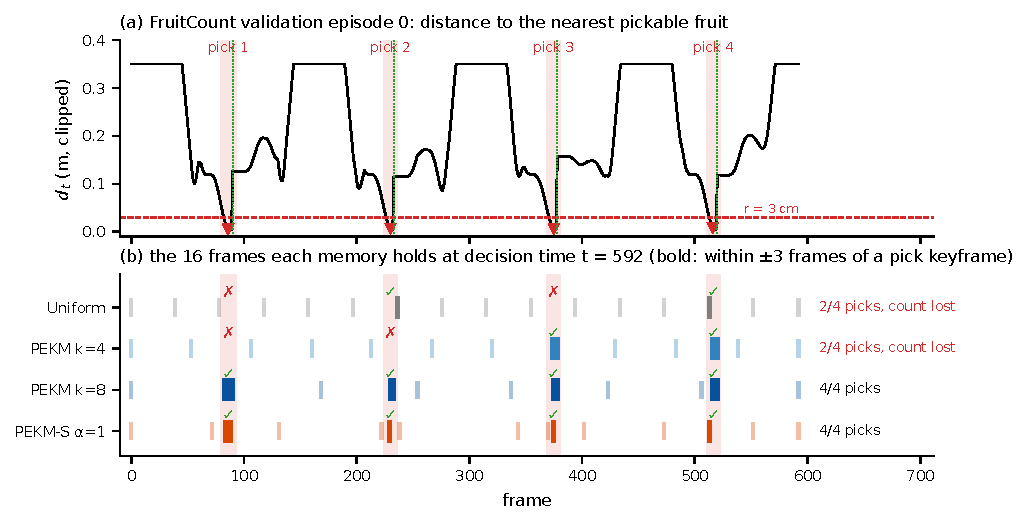
\includegraphics[width=\linewidth]{fig4_memory_timeline}
\caption{What a 16-frame memory actually holds. (a) TCP-to-fruit distance $d_t$ in the first FruitCount validation episode (four picks), with the detected picks and their $\pm3$-frame key windows (shaded), contact keyframes (triangles), the radius $r$ (dashed) and fruit detachments (dotted). (b) The frames held by each memory at the last decision ($t=592$); bold ticks lie within $\pm3$ frames of a contact or release keyframe, and \textcolor{green!50!black}{\checkmark}\,/\,\textcolor{red}{$\times$} marks whether each pick is covered. Uniform memory keeps picks 2 and 4 only because its grid happens to fall on them and misses picks 1 and 3, so the pick count is lost; \pekm\ with $k=4$ keeps the two most recent picks by construction, and $k=8$ and PEKM-S keep all four. Further examples are given in Supplementary Fig.~S1.}
\label{fig:timeline}
\end{figure}

\emph{Forgetting grows with operating time, as the coverage analysis predicts.} Over the 200 validation episodes (7884 decision--pick pairs), uniform memory at $B=16$ covers 97.8\% of completed picks in the first 200 frames, then 56.6\%, 40.8\% and only 26.4\% beyond 600 frames, and the most recent pick falls from 97.8\% to 21.7\% (Fig.~\ref{fig:theory}a,b). Equation~(\ref{eq:coverage}) predicts the measured coverage to within 0.012 at every budget (predicted / measured: 0.282 / 0.270 for $B=8$, 0.562 / 0.570 for $B=16$, 0.882 / 0.883 for $B=32$) and tracks its decay over time (Fig.~\ref{fig:theory}c): the failure is structural and cannot be tuned away. \pekm\ removes the dependence on time: $k=4$ and $k=8$ cover the most recent pick at every decision time, and $k=8$ covers at least 94.6\% of all completed picks even beyond 600 frames.

\begin{figure}[t]
\centering
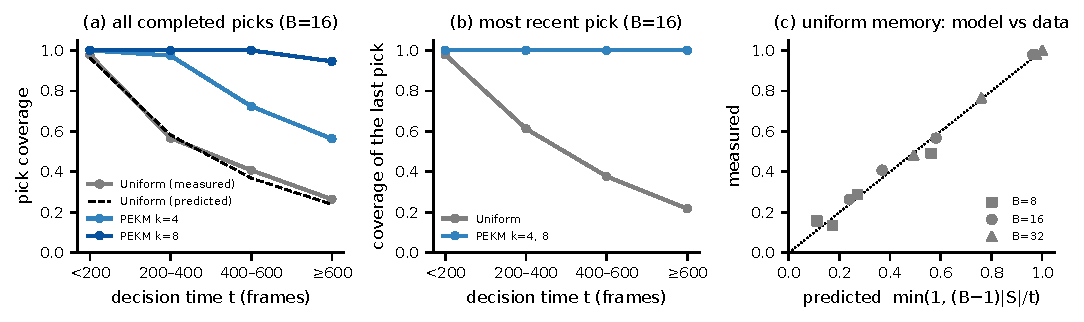
\includegraphics[width=\linewidth]{fig_coverage_theory}
\caption{Time-indexed memory forgets more the longer the robot works. (a) Coverage of all completed picks versus decision time at $B=16$: uniform memory (measured and predicted by Eq.~(\ref{eq:coverage})) and PEKM. (b) Coverage of the most recent pick. (c) Predicted versus measured coverage of uniform memory for every budget and decision-time bin.}
\label{fig:theory}
\end{figure}

\emph{\pekm\ retains recent picks by construction, without losing temporal context.} With $k=4$ the last two picks are always covered (picks 3 and 4 in Fig.~\ref{fig:timeline}) and overall coverage rises to 87.6\%; with $k=8$ coverage reaches 99.6\% and count recoverability 99.2\% (from 0.389 to 0.985 in FruitCount, from 0.485 to 1.000 in FruitOccludedRipe). The median gap between memory frames grows only from 14 to 17 frames (Fig.~\ref{fig:coverage}c). The soft variant concentrates six times more frames near fruits than U and covers older picks evenly, but at the cost of the most recent pick (0.814) and of temporal context (median gap 63 frames), which is why hard reservation is the main method. Increasing the cap to $k=12$ covers every pick, and an intermediate mixing weight ($\alpha=0.5$) trades the two effects without removing either (Table~\ref{tab:coverage}). \emph{Budget efficiency} follows: K4 with 8 frames (85.9\%) exceeds uniform memory with 16 frames and approaches it with 32 (88.3\%), and K8 with 16 frames (99.6\%) exceeds uniform memory with 32 (Fig.~\ref{fig:coverage}a), i.e.\ the same event information with a memory two to four times shorter.

\begin{table}[t]
\centering
\caption{Information retained by 16-frame memories (validation, both tasks; 5318 decisions, 7841 decision--pick pairs). Run cov.: at least one memory frame inside the pick's near run. Last / 2nd / 3rd: coverage of the most recent, second and third most recent pick. Near: fraction of memory frames with $d_t \le r$. Gap: median gap between memory frames (frames).}
\label{tab:coverage}
\footnotesize
\begin{adjustbox}{max width=\textwidth}\begin{tabular}{lcccccccc}
\toprule
Memory & Event cov. & Run cov. & Count rec. & Last & 2nd & 3rd & Near & Gap\\
\midrule
Uniform (U, K0) & 0.570 & 0.461 & 0.431 & 0.675 & 0.472 & 0.416 & 0.042 & 14\\
Recent & 0.080 & 0.069 & 0.046 & 0.145 & 0.000 & 0.000 & 0.049 & 209\\
Random & 0.432 & 0.364 & 0.329 & 0.533 & 0.351 & 0.231 & 0.040 & 41\\
PEKM $k=2$ & 0.729 & 0.681 & 0.579 & 1.000 & 0.430 & 0.336 & 0.085 & 17\\
\textbf{PEKM $k=4$} & \textbf{0.876} & \textbf{0.875} & \textbf{0.814} & \textbf{1.000} & \textbf{1.000} & 0.136 & 0.110 & 17\\
\textbf{PEKM $k=8$} & \textbf{0.996} & \textbf{0.995} & \textbf{0.992} & \textbf{1.000} & \textbf{1.000} & \textbf{1.000} & 0.123 & 17\\
PEKM $k=12$ & 1.000 & 1.000 & 1.000 & 1.000 & 1.000 & 1.000 & 0.124 & 17\\
PEKM-S $\alpha=0.5$ & 0.878 & 0.854 & 0.756 & 0.811 & 0.982 & 0.948 & 0.153 & 31\\
PEKM-S $\alpha=1$ & 0.897 & 0.873 & 0.770 & 0.814 & 1.000 & 1.000 & 0.265 & 63\\
\bottomrule
\end{tabular}\end{adjustbox}
\end{table}


\begin{figure}[t]
\centering
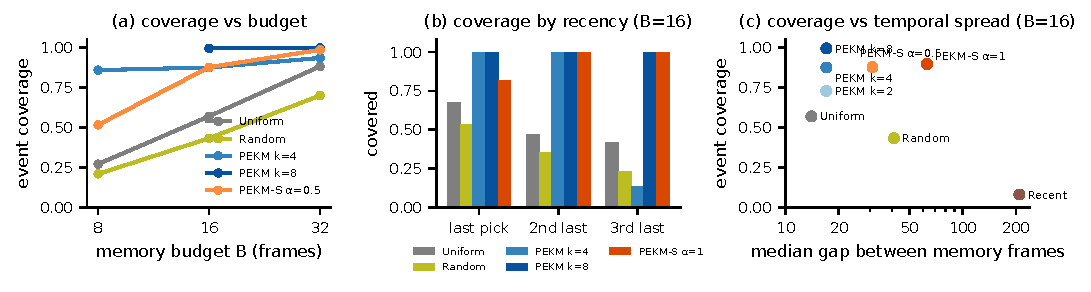
\includegraphics[width=\linewidth]{fig7_memory_coverage}
\caption{Memory coverage. (a) Event coverage versus budget $B$. (b) Coverage of the last three picks at $B=16$. (c) Event coverage versus median gap between memory frames: PEKM raises coverage without sacrificing temporal resolution.}
\label{fig:coverage}
\end{figure}

\subsection{Fruit segmentation with SAM (RQ5)}
\label{sec:res_sam}
Table~\ref{tab:sam} and Fig.~\ref{fig:sam} compare fruit segmentation on 8644 rendered validation images (13{,}424 front-camera and 4877 wrist-camera instances).

\emph{Prompted SAM gives the most accurate masks.} \fdm\ reaches an instance F1 of 0.991 (front) and 0.983--0.984 (wrist), with tighter masks than colour thresholding (IoU 0.974--0.978 versus 0.945), which matters because fruit centres are estimated from the mask, and recovers more partially hidden fruits (recall 0.967--0.976 versus 0.952 at 25--75\% visibility, 0.633--0.688 versus 0.615 below 25\%). Ripeness is correct for every matched instance with all methods.

\emph{Prompts are essential, and a small backbone suffices.} Without prompts, SAM-AUTO is precise (0.994--0.996) but misses partially hidden fruits (recall 0.57--0.62 at 25--75\% visibility, 0.21--0.26 below 25\%) and is four to seven times slower (395--626~ms per image). The three \fdm\ backbones have the same F1 (0.991) and differ by at most 0.004 in IoU, while latency grows from 94~ms (ViT-B) to 309~ms (ViT-H); since SAM runs once per episode, ViT-B is the practical choice for embedded platforms. With ground-truth boxes, SAM reaches F1 0.999 and a recall of 0.899 below 25\% visibility, so the remaining gap lies in prompting barely visible fruits, not in SAM's masks.

\emph{Illumination locates the component that must adapt.} We re-rendered every third frame under overcast or dusk, direct sun and warm low sun with the colour thresholds kept as calibrated (Table~\ref{tab:light}; Fig.~\ref{fig:sam}c), using a gamma-darkened ($0.55\,x^{1.2}$), a brightened ($1.35\,x^{0.85}$) and a warm colour cast (channel gains 1.12 / 1.00 / 0.80). Given correct box prompts, SAM's F1 stays at 0.999 and its IoU at 0.979 under all three conditions, whereas fixed colour thresholds do not transfer (F1 below 0.1) and \fdm\ inherits this through its prompts. The component to adapt for field use is therefore the prompt generator, which can be replaced by an illumination-normalized colour model or a learned detector without changing SAM, the anchors or the policy. \tbd{Optional: colour-normalized or learned prompt source as an additional row.}

\begin{table}[t]
\centering
\caption{Fruit instance segmentation and ripeness on rendered validation images (8644 images; 13{,}424 front and 4877 wrist instances). F1 at IoU $\ge 0.5$. IoU: mean over matched front-camera instances. R (vis.): front-camera recall by visible fraction (418 instances at 25--75\%, 109 below 25\%). Latency: median per front image on one L20 GPU. SAM-AUTO was evaluated on every 5th frame.}
\label{tab:sam}
\footnotesize
\begin{adjustbox}{max width=\textwidth}\begin{tabular}{llccccccc}
\toprule
Method & Backbone & F1 front & F1 wrist & IoU & R (25--75\%) & R ($<$25\%) & Ripeness & ms/img\\
\midrule
HSV thresholds & -- & 0.990 & 0.980 & 0.945 & 0.952 & 0.615 & 1.000 & 1.4\\
SAM-AUTO & ViT-B & 0.937 & 0.983 & 0.979 & 0.573 & 0.263 & 1.000 & 395\\
SAM-AUTO & ViT-H & 0.941 & 0.981 & 0.970 & 0.618 & 0.211 & 1.000 & 626\\
\fdm & ViT-B & \textbf{0.991} & \textbf{0.984} & 0.974 & 0.967 & 0.633 & 1.000 & 94\\
\fdm & ViT-L & \textbf{0.991} & \textbf{0.984} & \textbf{0.978} & \textbf{0.976} & \textbf{0.688} & 1.000 & 195\\
\fdm & ViT-H & \textbf{0.991} & 0.983 & 0.975 & 0.971 & 0.651 & 1.000 & 309\\
\midrule
SAM-GTBOX (upper bound) & ViT-H & 0.999 & 0.999 & 0.980 & 1.000 & 0.899 & 1.000 & --\\
\bottomrule
\end{tabular}\end{adjustbox}
\end{table}

\begin{table}[t]
\centering
\caption{Segmentation F1 under illumination shifts (front and wrist cameras together; 6396 instances per shifted condition, 18{,}301 nominal). Colour thresholds as calibrated under nominal lighting; SAM backbone ViT-H.}
\label{tab:light}
\footnotesize
\begin{adjustbox}{max width=\textwidth}\begin{tabular}{lcccc}
\toprule
Condition & HSV thresholds & \fdm\ (colour prompts) & SAM-GTBOX F1 & SAM-GTBOX IoU\\
\midrule
Nominal & 0.987 & 0.989 & 0.999 & 0.979\\
Direct sun (bright) & 0.079 & 0.096 & 0.999 & 0.979\\
Overcast / dusk (dark) & 0.000 & 0.000 & 0.999 & 0.979\\
Low sun (warm) & 0.018 & 0.031 & 0.999 & 0.979\\
\bottomrule
\end{tabular}\end{adjustbox}
\end{table}

\begin{figure}[t]
\centering
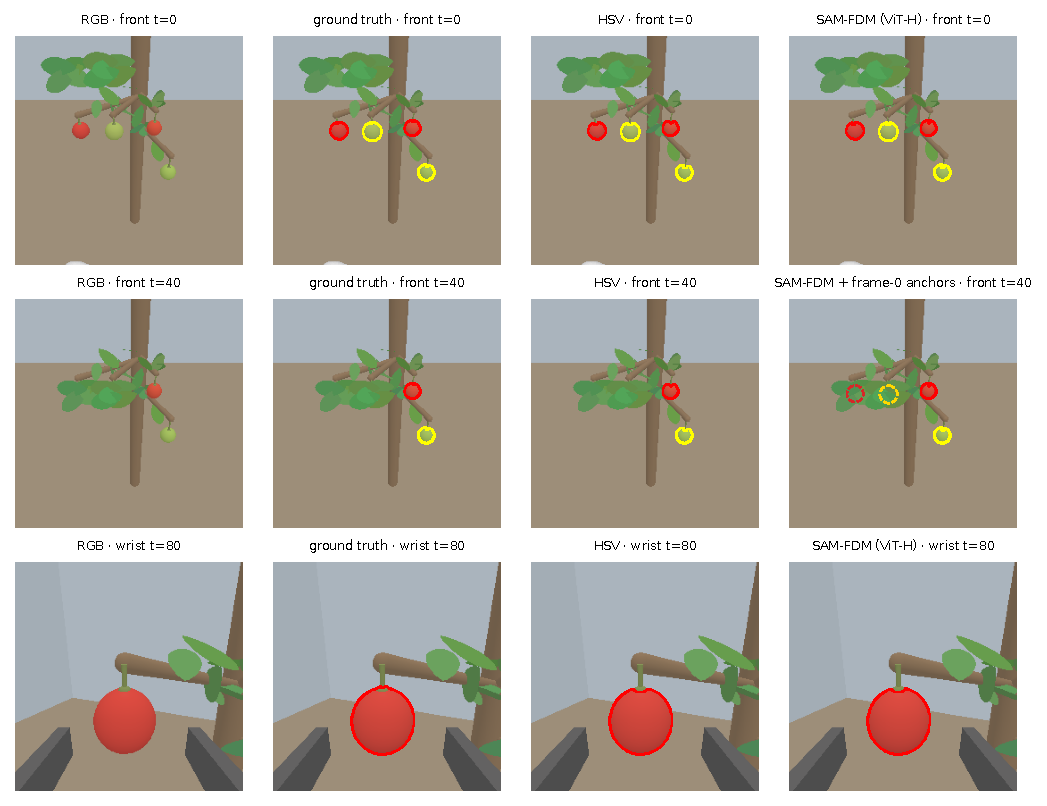
\includegraphics[width=0.74\linewidth]{fig8a_sam_qualitative}\\[2pt]
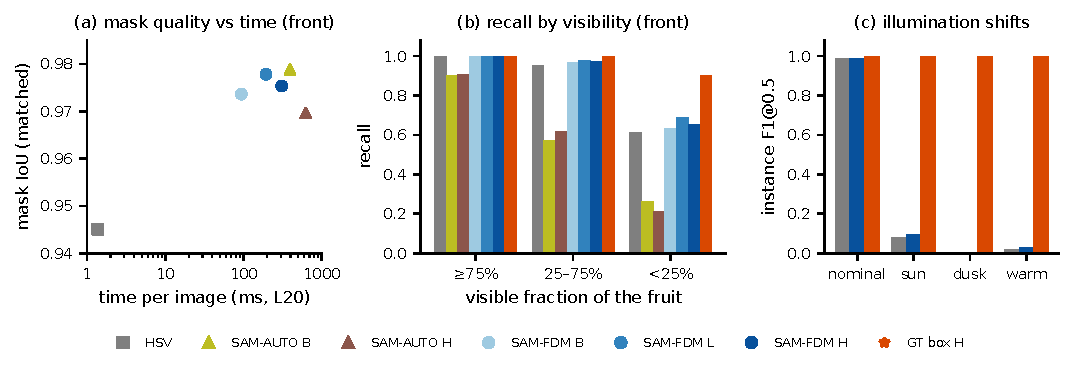
\includegraphics[width=\linewidth]{fig8b_sam_quantitative}
\caption{Fruit segmentation. Top: a FruitOccludedRipe validation episode before the gust (front, $t=0$), after it (front, $t=40$) and at contact (wrist, $t=80$); columns show the image, ground truth, HSV thresholds and \fdm\ (ViT-H), with red contours for ripe and yellow for unripe fruits. At $t=40$, dashed circles are the frame-0 anchors, which keep the two leaf-hidden fruits in memory. Bottom: (a) mask IoU versus latency; (b) front-camera recall by visible fraction; (c) F1 under illumination shifts.}
\label{fig:sam}
\end{figure}

\subsection{From RGB-D images to event memory (RQ6)}
\label{sec:res_chain}
Table~\ref{tab:chain} evaluates the complete chain on the 199 validation episodes using only the recorded front RGB-D frames, forward kinematics and the gripper state, with no simulator ground truth (per-task results with the K8 memory in Supplementary Table~S3).

\emph{Anchors, distances and events.} Frame-0 anchors recover 99.8\% of fruits with 99.5\% precision, a median localization error of 0.48~cm (90th percentile 0.58~cm), below a fifth of the fruit radius, and error-free ripeness; all 138 ripe fruits that the gust later hides have an anchor (Section~\ref{sec:res_anchor}). The perceived distance has a median near-range error of 0.34~cm (90th percentile 0.48~cm), well inside the accuracy specification above. Events detected from $\hat d_t$ match the ground truth exactly (F1 1.000, count exact in every episode, release error 0 frames), and the \pekm\ memories recover every ground-truth keyframe (Jaccard 0.948 for $k=4$, 0.941 for $k=8$, the differences being contact frames shifted by one or two frames). Consumer-grade depth noise leaves all results unchanged.

\emph{Grasp evidence closes the visual blind spot, and anchors beat per-frame detection.} With depth vacancy alone, the arm and the carried fruit occlude the anchor during carrying, so the release keyframe is late by a median of 16 frames and the memory Jaccard drops to 0.685; the nearly free gripper-holding cue removes the delay. Without anchors, the carried fruit is still detected as the nearest fruit: the release error grows to 52 frames and spurious events appear (precision 0.821, count exact in 62\% of episodes; 0.759 and 46\% in FruitCount), and even with hysteresis (precision 0.942) the memory Jaccard remains 0.421 (Fig.~\ref{fig:chain}).

\begin{table}[t]
\centering
\caption{Events and memory from perceived distances (199 validation episodes; plain detector, hysteresis in parentheses). Dist.\ err.: median / 90th-percentile error of $\hat d_t$ where $d_t \le 10$ cm. Rel.\ err.: median release-keyframe error (frames). Jaccard and KF recall: agreement of the K4 memory with the GT memory. For K8, Jaccard is 0.941 / 0.941 / 0.660 / 0.730 / 0.363 and KF recall 1.000 / 1.000 / 0.847 / 0.882 / 0.782 for the rows below GT.}
\label{tab:chain}
\footnotesize
\begin{adjustbox}{max width=\textwidth}\begin{tabular}{lcccccccc}
\toprule
Distance source & Dist.\ err.\ (cm) & P & R & F1 & Count & Rel.\ err. & Jaccard & KF recall\\
\midrule
GT (upper bound) & 0 / 0 & 1.000 & 1.000 & 1.000 & 1.00 & 0 & 1.000 & 1.000\\
\textbf{\fdm\ (ours)} & \textbf{0.34 / 0.48} & \textbf{1.000} & \textbf{1.000} & \textbf{1.000} & \textbf{1.00} & \textbf{0} & \textbf{0.948} & \textbf{1.000}\\
\fdm\ + depth noise & 0.31 / 0.46 & 1.000 & 1.000 & 1.000 & 1.00 & 0 & 0.948 & 1.000\\
Depth-only & 0.39 / 10.76 & 1.000 & 1.000 & 1.000 & 1.00 & 16 & 0.685 & 0.845\\
Post-gust anchors & 0.39 / -- & 1.000 & 0.743 & 0.853 & 0.50 & 0 & 0.741 & 0.880\\
Per-frame & 0.39 / 12.79 & 0.821 (0.942) & 1.000 & 0.902 (0.970) & 0.62 (0.85) & 52 & 0.421 & 0.755\\
\bottomrule
\end{tabular}\end{adjustbox}
\end{table}

\begin{figure}[t]
\centering
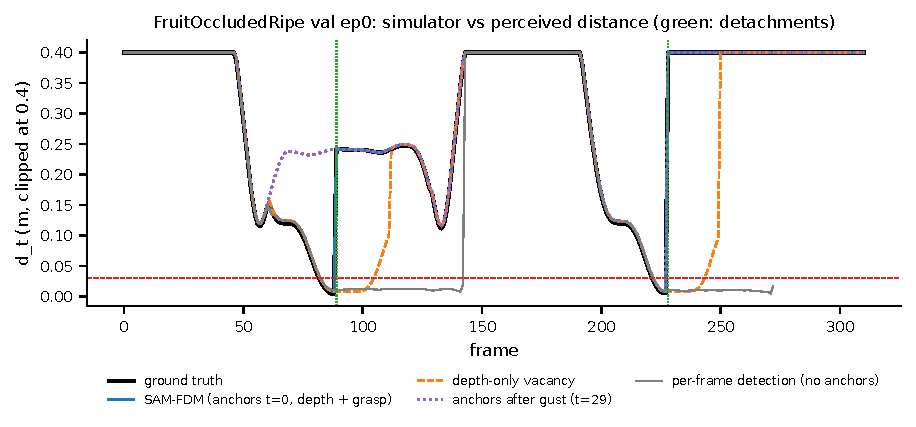
\includegraphics[width=0.82\linewidth]{fig_e6_perceived_distance}
\caption{Perceived versus ground-truth distance in one FruitOccludedRipe episode (vertical lines: detachments). \fdm\ follows the ground truth; depth-only vacancy confirms detachment late, post-gust anchors miss the hidden ripe fruit, and per-frame detection tracks the carried fruit.}
\label{fig:chain}
\end{figure}

\subsection{Spatial memory before occlusion is a precondition for event memory (RQ6)}
\label{sec:res_anchor}
The perception chain above builds its anchors at frame 0, before the wind gust. To isolate the role of this spatial memory, we rebuilt the anchors at frame 29, after the gust, with everything else unchanged, i.e.\ the same segmentation, depth, grasp evidence, detector and memory. Table~\ref{tab:anchors} and Fig.~\ref{fig:anchor} report the result per task.

\emph{Hidden ripe fruits disappear from memory.} In FruitOccludedRipe, post-gust anchors recover only 56.8\% of the fruits, against 99.6\% before the gust, and \emph{none} of the 138 ripe fruits that the leaves hide receives an anchor (0\% against 100\%). Over both tasks, this is the drop from 99.8\% to 78.3\% anchor recall. The anchors that are built are as good as before: precision 0.989 versus 0.994, localization error 0.49 versus 0.48~cm, ripeness error-free in both cases. The degradation therefore concerns \emph{when} the spatial memory is formed, not \emph{how accurately} it is measured.

\emph{The loss propagates to events and to the policy's memory.} Without an anchor, the robot's approach to a hidden ripe fruit produces no distance minimum. The median near-range distance error grows from 0.35 to 5.78~cm, and in more than a tenth of the near-range frames no fruit is perceived at all. Event recall falls from 1.000 to 0.450: 138 of the 251 picks go undetected, as many as there are leaf-hidden ripe fruits. Not a single FruitOccludedRipe episode keeps the correct pick count (0.00 versus 1.00). The K4 memory recovers only 73.1\% of its ground-truth keyframes (Jaccard 0.493 versus 0.948), so the frames reserved for picks would be spent on the wrong moments.

\emph{The failure is silent, and specific to occlusion.} Precision stays at 1.000 because every detected event is real, so a precision-based check would not reveal that half of the picks are missing. In FruitCount, where no fruit is hidden by foliage, frame-0 and frame-29 anchors give identical results in every metric, which confirms that the loss is caused by occlusion and not by the change of anchoring frame. Consumer-grade depth noise leaves the frame-0 results unchanged (localization error 0.45~cm). Remembering \emph{where} a fruit is, perceived while it was visible, is a precondition for remembering \emph{that} it was picked. In practice, a harvesting system should build its spatial memory when it first faces a plant, before its own motion, wind or leaf contact occlude the fruits, and keep that memory persistent.

\begin{table}[t]
\centering
\caption{Spatial memory before versus after occlusion (\fdm, ViT-H; 199 validation episodes; plain detector). Anchors are built at frame 0 (before the gust) or at frame 29 (after it); all other components are unchanged. Hidden ripe: leaf-hidden ripe fruits with an anchor. Dist.\ err.: median error of $\hat d_t$ where $d_t \le 10$ cm. Count: fraction of episodes with the exact pick count. Jaccard and KF recall: agreement of the K4 memory with the ground-truth memory.}
\label{tab:anchors}
\footnotesize
\setlength{\tabcolsep}{4pt}
\begin{adjustbox}{max width=\textwidth}\begin{tabular}{llcccccccccc}
\toprule
 & & \multicolumn{4}{c}{Spatial memory (anchors)} & & \multicolumn{3}{c}{Picking events} & \multicolumn{2}{c}{K4 memory}\\
\cmidrule(lr){3-6}\cmidrule(lr){8-10}\cmidrule(lr){11-12}
Task & Anchors at & Recall & Prec. & Loc.\ err.\ (cm) & Hidden ripe & Dist.\ err.\ (cm) & Recall & F1 & Count & Jaccard & KF recall\\
\midrule
FruitOccludedRipe & \textbf{frame 0 (ours)} & \textbf{0.996} & 0.994 & 0.48 & \textbf{138 / 138} & \textbf{0.35} & \textbf{1.000} & \textbf{1.000} & \textbf{1.00} & \textbf{0.948} & \textbf{1.000}\\
 & frame 0 + depth noise & 0.996 & 0.994 & 0.45 & 138 / 138 & 0.32 & 1.000 & 1.000 & 1.00 & 0.948 & 1.000\\
 & frame 29 & 0.568 & 0.989 & 0.49 & 0 / 138 & 5.78 & 0.450 & 0.621 & 0.00 & 0.493 & 0.731\\
\midrule
FruitCount & frame 0 (ours) & 1.000 & 0.996 & 0.48 & -- & 0.33 & 1.000 & 1.000 & 1.00 & 0.947 & 1.000\\
(control) & frame 29 & 1.000 & 0.996 & 0.48 & -- & 0.33 & 1.000 & 1.000 & 1.00 & 0.947 & 1.000\\
\midrule
Both tasks & frame 0 (ours) & \textbf{0.998} & 0.995 & 0.48 & \textbf{138 / 138} & 0.34 & \textbf{1.000} & \textbf{1.000} & \textbf{1.00} & 0.948 & 1.000\\
 & frame 29 & 0.783 & 0.993 & 0.49 & 0 / 138 & 0.39 & 0.743 & 0.853 & 0.50 & 0.741 & 0.880\\
\bottomrule
\end{tabular}\end{adjustbox}
\end{table}

\begin{figure}[t]
\centering
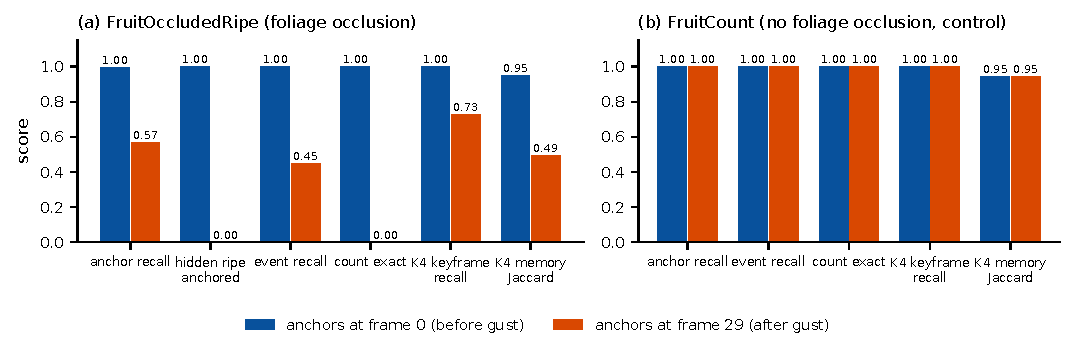
\includegraphics[width=\linewidth]{fig_anchor_timing}
\caption{How the timing of spatial memory propagates to event memory. Anchors built before the gust (frame 0, blue) or after it (frame 29, orange), with all other components unchanged. (a) In FruitOccludedRipe, post-gust anchoring loses every leaf-hidden ripe fruit, and the loss carries through to the detected picks, the pick count and the frames reserved in the K4 memory. (b) In FruitCount, without foliage occlusion, the two anchoring times are indistinguishable.}
\label{fig:anchor}
\end{figure}

\subsection{Closed-loop harvesting (RQ7)}
\label{sec:res_closed}
Table~\ref{tab:closed} reports closed-loop results on validation episodes 50--99 (150 trials per task and condition). \tbd{Main results after the sealed evaluation: success of K0/K4/K8 per task with paired differences, 95\% CIs and Holm-adjusted p-values; process metrics; stratification by quota $N$ (2 / 3 / 4--5); validity gates (engineering errors, complete blocks, per-decision frame audit).}

\begin{table}[t]
\centering
\caption{Closed-loop harvesting on validation episodes 50--99 (3 seeds; 150 trials per cell). Paired differences with 95\% bootstrap CIs; Holm-adjusted p-values over the primary family.}
\label{tab:closed}
\footnotesize
\begin{adjustbox}{max width=\textwidth}\begin{tabular}{llcccccc}
\toprule
Task & Memory & Success & Completion & Over-/wrong-pick & Drop & Steps & $\Delta$ vs K0 [95\% CI]\\
\midrule
FruitCount & K0 (uniform) & \tbd{} & \tbd{} & \tbd{} & \tbd{} & \tbd{} & --\\
 & K4 (PEKM) & \tbd{} & \tbd{} & \tbd{} & \tbd{} & \tbd{} & \tbd{}\\
 & K8 (PEKM) & \tbd{} & \tbd{} & \tbd{} & \tbd{} & \tbd{} & \tbd{}\\
FruitOccludedRipe & K0 (uniform) & \tbd{} & \tbd{} & \tbd{} & \tbd{} & \tbd{} & --\\
 & K4 (PEKM) & \tbd{} & \tbd{} & \tbd{} & \tbd{} & \tbd{} & \tbd{}\\
 & K8 (PEKM) & \tbd{} & \tbd{} & \tbd{} & \tbd{} & \tbd{} & \tbd{}\\
\bottomrule
\end{tabular}\end{adjustbox}
\end{table}

\subsection{Ablations and counterfactual controls (RQ7)}
\label{sec:res_ablation}
Table~\ref{tab:ablation} lists the test-time ablations of the K4 policy under the same paired protocol. \tbd{Ablation results: keyframe cap, radius, hard vs soft selection, signal source (GT, \fdm, noisy), counterfactual controls EVU/EVR/EVA, keyframe composition, training data.}

\begin{table}[t]
\centering
\caption{Ablations (test-time variants of the K4 policy unless noted; paired differences to the default configuration).}
\label{tab:ablation}
\footnotesize
\begin{adjustbox}{max width=\textwidth}\begin{tabular}{llcc}
\toprule
Factor & Setting & FruitCount $\Delta$ & FruitOccludedRipe $\Delta$\\
\midrule
Keyframe cap $k$ (trained) & 0 / 4 / 8 & \tbd{} & \tbd{}\\
Radius $r$ & 1 / 3 / 5 cm & \tbd{} & \tbd{}\\
Selection & hard (PEKM) / soft (PEKM-S, $\alpha=0.5$) & \tbd{} & \tbd{}\\
Signal source & GT / \fdm\ / GT + 1 cm noise & \tbd{} & \tbd{}\\
Counterfactual & EV / EVU / EVR / EVA & \tbd{} & \tbd{}\\
Keyframes & contact / release / both & \tbd{} & \tbd{}\\
Training data & clean (C0) / clean + DART-H (K0) & \tbd{} & \tbd{}\\
\bottomrule
\end{tabular}\end{adjustbox}
\end{table}

\subsection{Open-loop accuracy and closed-loop drift (RQ8)}
\label{sec:res_dart}
Table~\ref{tab:openloop} evaluates a uniform-memory policy trained on clean demonstrations in open loop, i.e.\ teacher-forced at the demonstrated states. Its median TCP errors are 1.7--2.4~cm at the end of a 16-step chunk and 0.7--1.1~cm near the fruit, an order of magnitude below the motion within a chunk, and it agrees with the demonstrated gripper direction in 98--99.5\% of decisions. Training and validation errors are nearly identical, so the policy generalizes to unseen layouts at the demonstrated states. In closed loop, however, small deviations accumulate into states that clean demonstrations do not cover, the covariate shift that DART-H targets; its perturbations (median 2.5~cm) match the scale of the open-loop errors. \tbd{Closed-loop C0 vs K0 comparison: success, harvest completion, failure modes.}

\begin{table}[t]
\centering
\caption{Open-loop (teacher-forced) accuracy of a uniform-memory policy trained on clean demonstrations (10 episodes per set). TCP error at horizons 1, 8 and 16 of the action chunk; near: horizon 16 while $d_t \le 10$ cm.}
\label{tab:openloop}
\footnotesize
\begin{adjustbox}{max width=\textwidth}\begin{tabular}{llccc}
\toprule
Set & Task & TCP error h1 / h8 / h16 (cm) & Near h16 (cm) & Gripper agreement\\
\midrule
Train & FruitCount & 0.44 / 1.23 / 1.83 & 0.75 & 99.5\%\\
Train & FruitOccludedRipe & 0.42 / 1.25 / 1.66 & 0.70 & 99.2\%\\
Validation & FruitCount & 0.51 / 1.37 / 2.38 & 1.14 & 98.0\%\\
Validation & FruitOccludedRipe & 0.40 / 1.32 / 1.75 & 0.78 & 98.9\%\\
\bottomrule
\end{tabular}\end{adjustbox}
\end{table}

\subsection{Memory content matters for VLA policies (supporting evidence)}
\label{sec:res_general}
The premise of this work, that the content of a fixed-budget memory influences a VLA policy, was verified on a general manipulation-memory benchmark (\tbd{cite RoboMME}) with the base policy, under sealed protocols with paired bootstrap and Holm adjustment (Table~\ref{tab:general}). Removing the history memory collapses success on a pattern-recall task from 66.7\% to 1.7\%, and halving the budget from 32 to 16 frames reduces it from 64.4\% to 26.7\%. Replacing a single memory slot changes the action loss with a slot-ranking reliability of 0.97--0.99 across four tasks: within a fixed budget, the choice of frames matters, which is exactly the decision that \pekm\ makes using the harvesting structure. \tbd{Generalization: success by quota $N$ and on unseen layouts from E7.}

\begin{table}[t]
\centering
\caption{Memory ablations of the base VLA on a general manipulation-memory benchmark (paired bootstrap, Holm-adjusted).}
\label{tab:general}
\footnotesize
\begin{adjustbox}{max width=\textwidth}\begin{tabular}{>{\raggedright\arraybackslash}p{4.8cm}>{\raggedright\arraybackslash}p{8.2cm}}
\toprule
Intervention & Result\\
\midrule
No history memory (pattern-recall task) & 66.7\% $\rightarrow$ 1.7\% ($-65.0$ pp, 95\% CI [$-81.7$, $-46.7$], $p<0.001$)\\
No memory (video-swap task) & $-11.7$ pp (95\% CI [$-20.0$, $-3.3$], $p=0.006$)\\
Budget 32 $\rightarrow$ 16 frames (pattern recall) & 64.4\% $\rightarrow$ 26.7\% ($-37.8$ pp, $p<0.001$)\\
Single-slot replacement (counterfactual action loss) & Slot-ranking reliability 0.97--0.99 over four tasks; cross-fitted relative gain 2.5--12.4\%\\
\bottomrule
\end{tabular}\end{adjustbox}
\end{table}

\subsection{Run-time cost (RQ8)}
\label{sec:res_cost}
At $t=1000$ frames, one \pekm\ selection takes 117~$\mu$s on a CPU core (39~$\mu$s for uniform sampling), negligible against one VLA inference (\tbd{VLA latency, ms}), and the memory footprint and inference cost of the policy are those of the uniform baseline, since the number of frames is unchanged. \fdm\ runs SAM once per episode (94 / 195 / 309~ms for ViT-B / L / H on one L20 GPU), and its per-frame work, projecting a few anchors and reading depth and gripper state, takes well under a millisecond. Detection itself is a threshold comparison per frame.
